\documentclass[12pt, a4paper]{article}
\usepackage[utf8]{inputenc}
\usepackage{hyperref}
\usepackage[dvipsnames]{xcolor}
\usepackage{graphicx}
\usepackage{listings}
\usepackage{float}
\usepackage{natbib}
\usepackage{acronym}

\graphicspath{{images/}}

% don't allow to split words over separate lines
\hyphenpenalty 10000
\exhyphenpenalty 10000
\raggedright

\renewcommand{\figurename}{Figur}



\title{Function as a Service}
\author{Xiang Rong Lin}
\date{27.11.2021}

\begin{document}

\maketitle



\newpage
\tableofcontents

\newpage

\section{Einleitung}
bli bla blub

\section{Grundlagen}
% stark kürzen
\subsection{Cloud computing}
Cloud computing wird vom \ac{NIST} als \cite[ein Modell zur Ermöglichung eines allgegenwärtigen, bequemen und bedarfsgerechten Netzzugang zu einem gemeinsamen Pool konfigurierbarer Rechenressourcen die schnell bereitgestellt und freigegeben werden können mit minimalem Verwaltungsaufwand oder Interaktion mit dem Dienstanbieter]{mell2011nist}.
In dieser Definition gibt es 5 wesentliche Merkmale, 3 Service Modelle und 4 Bereitstellungsmethoden.

\subsection{Merkmale}
Eine kurze Zusammenfassung von \ac{NIST}\cite{mell2011nist}
\subsubsection{On-demand self-service}
Ein Benutzer kann sich selbstständig und automatisiert Ressourcen bereitstellen oder abbestellen ohne eine jegliche Interaktion mit einem Menschen. 

\subsubsection{Broad network access}
Diese Ressourcen sind über ein standardisiertes Interface erreichbar. Dies ist meist das Internet per HTTP.

\subsubsection{Resource pooling}
Der Anbieter dieser Ressourcen verfügt über einen Pool, welche entsprechend der Kundenwünsche zugewiesen werden. Dies passiert in Form von virtuellen Maschinen oder auch Containern.

\subsubsection{Rapid elasticity}
Ressourcen können sehr schnell hinzugefügt und auch wieder entfernt.

\subsubsection{Measured service}
Der Verbrauch von Ressourcen kann sehr genau abgerechnet werden, z.B. in Millisekundenbereich an verwendeter CPU Zeit.

\subsection{Servicemodelle}
In der initialen Definition aus 2011 wurden die 3 Modelle \ac{SaaS}, \ac{PaaS} und \ac{IaaS} beschrieben \cite{mell2011nist}. Inzwischen gibt es eine Vielzahl an Angeboten wie zum Beispiel \ac{BaaS} oder \ac{FaaS}. Es ist auch schon die Rede von \ac{XaaS}, also dass man alles als Service anbieten kann.
\begin{figure}
    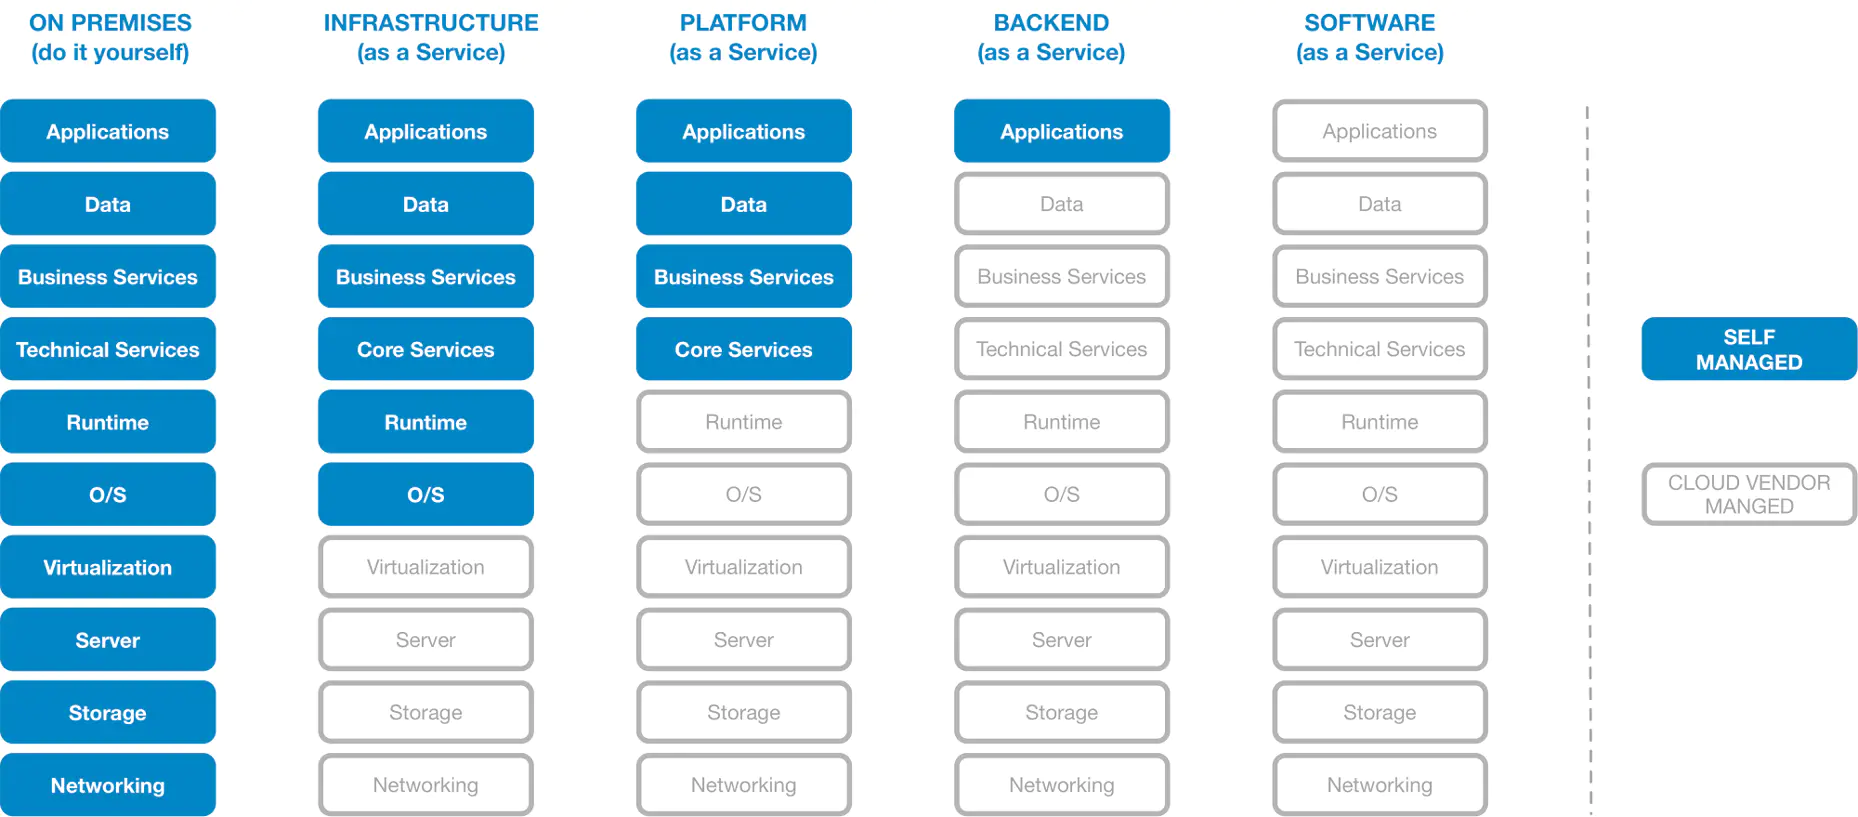
\includegraphics[width=\textwidth, height=\textheight,keepaspectratio]{cloud_service_models.png}
    \caption{Cloud service models}
    \cite{serverless2017roewekamp}
\end{figure}
An obiger Grafik sieht man dass man von \ac{IaaS} über \ac{PaaS} hin zu \ac{SaaS} immer mehr direkt vom Anbieter bereit gestellt kriegt und immer weniger selbst managen muss.
Die neuen Modelle stellen somit nur einen anderen Schnitt der Verantwortlichkeiten dar.

\section{Was ist \ac{FaaS}?}
\ac{FaaS} ist einer der neueren Aufteilungen der Verantwortlichkeiten zwischen einem selbst und dem Anbieter.
In dieser neuen Form muss man selbst nur noch die Businesslogik implementieren und der Anbieter kümmert sich um den Betrieb in der Cloud.
Genauer beschrieben hatte man zuvor drei unterschiedliche Aufgabenbereiche\cite{serverless2017roewekamp}:
\begin{enumerate}
    \item Ablaufsteuerung und lokale Logik
    \item standardisierte Geschäftslogik
    \item individuelle Geschäftslogik
\end{enumerate}
Von diesen übernimmt der Anbieter die ersten beiden, sodass man sich nur noch um die individuelle Geschäftslogik kümmern muss. 
\newline
Oft werden die Begriffe Serverless und \ac{FaaS} austauschbar verwendet was falsch ist.
IBM beschreibt den wichtigen Unterschied, dass \ac{FaaS} ein Ausschnitt von Serverless ist\cite{faas2019ibm}.
Wo man bei Serverless nur compute Ressourcen erhält, beinhaltet Serverless auch storage, database, messaging und vieles mehr.

\subsection{Serverless}
Serverless bietet außerhalb von Berechnungskapazitäten unter anderem auch Speicher-, Datenbank- und Benachrichtigungsservices an. \footnote{https://www.ibm.com/cloud/learn/faas 27.11.21}
FaaS ist somit nur ein Teil von Serverless, werden fälschlicherweise austauschbar verwendet.

% \newpage

\section{Wie verwendet man \ac{FaaS}?}
Die Funktionsweise aus Sicht des Anwendungsentwicklers wird im \cite[Developer Guide von \ac{AWS}]{awsLambda_devGuide} sehr detailliert dargestellt.
Grundlegend muss man selbst nur die Funktion implementieren und einen entsprechenden Trigger festlegen.

Im Java Beispiel implementiert man die Funktion indem man eines der unteren beiden Interfaces implementiert.

\begin{figure}[h]
    \lstinputlisting[language=Java]{code/RequestHandler.java}
    \caption{RequestHandler.java}
    % https://github.com/aws/aws-lambda-java-libs/blob/master/aws-lambda-java-core/src/main/java/com/amazonaws/services/lambda/runtime/RequestHandler.java
\end{figure}

\begin{figure}[h]
    \lstinputlisting[language=Java]{code/RequestStreamHandler.java}
    \caption{RequestStreamHandler.java}
    % https://github.com/aws/aws-lambda-java-libs/blob/master/aws-lambda-java-core/src/main/java/com/amazonaws/services/lambda/runtime/RequestStreamHandler.java
\end{figure}
 
Der Eingabetyp muss ein primitive Datentyp, String, ein \ac{POJO}, eine Collection davon, ein Stream oder ein AWS spezifisches Event sein und wird per Konfiguration in einer `Event.json' definiert.
Benötigt man zusätzlich noch Zugriff auf Datenbanken, Dateisystem oder andere Services bietet \ac{AWS} Lambda noch zusätzliche Bibliotheken für den Zugriff.
\newline\newline
Als Trigger kann man HTTP Anfragen, Queue Nachrichten, Streams oder andere \ac{AWS} Services verwendet werden.
Tritt nun eines dieser Ereignisse ein, so wird der Handler aufgerufen.
Dies kann synchron ablaufen in welchen Fall das Ereignis direkt vom Client an den Handler weitergegeben wird.
Dies wird beispielsweise bei HTTP Anfragen oft benötigt, da der Benutzer am anderen Ende aktiv auf die Antwort wartet.
\newline
Die bevorzugte Arbeitsweise ist aber asynchron.
Hier wird das Event in eine Warteschlange eingereiht und der Client wartet nicht auf eine Antwort.
Diese Events werden dann nach und nach von den Handlern abgearbeitet.
Diese asynchrone arbeitsweise wird auch als \emph{Event-Driven Architecture} bezeichnet, was viele Vorteile sowie Nachteile mit sich bringt\cite{awsEventDrivenArchitecture}.
Viele davon sind allgemein gültig und nicht nur auf für \ac{FaaS} bezogen.
Die wichtigsten davon sind aber dass die Komponenten unabhängig voneinander entwickelt, betrieben und skaliert werden können.

% Vendor Lock In

\section{Wie funktioniert FaaS intern?}
Wie kann man aber selber \ac{FaaS} anbieten?
\newline
Hierfür kann man sich das Open Source Projekt \cite[OpenFaaS]{openfaas_github} genauer anschauen.
Es verspricht eine viel weniger restriktive Lösung gegenüber den kommerziellen Lösungen von Amazon, Google und co.
Kubernetes wird als Grundtechnologie verwendet, was einem erlaubt jegliche Anwendung zu verwenden, die in einem Container laufen kann.
Mit Kubernetes kommt auch die automatische skalierung, aber vor allem auch die Unabhängigkeit von Cloud Anbieter, da Kubernetes verglichen mit \ac{FaaS} ein viel älteres und somit standardisierteres Modell ist.
\newline
Vor allem hat man aber vollen Zugriff zum Source Code und kann anhand des \emph{Template Store}\cite{openfaas_templateStore} genau sehen wie ein \ac{FaaS} Provider implementiert ist.
Die Templates bestehen aus 4 Teilen aus denen ein lauffähiges Docker Images erstellt wird, welche am Java 11 HTTP Beispiel \cite{openfaas_templateStore_java11} hier aufgeführt werden.
\newline
\newline
Als erstes hat man das Dockerfile mit der die Applikation gebaut wird und anschließend in einer minimalen Laufzeitumgebung gestartet wird.
\newline
Dabei erhält die Applikation Anfragen nicht direkt sondern über den \emph{of-watchdog}\cite{openfaas_ofWatchdog}.
Dies ist ein HTTP Server von OpenFaaS, der als reverse proxy zum ausführen der Funktionen dient.
Es gibt verschiedene Operationsmodi die entweder dynamisch skaliert werden können über Systemprozesse und dann über STDIO kommunizieren oder in unseren Fall eine 1:1 Beziehung haben und über http auf dem localhost kommunizieren.
Der Vorteil des \emph{of-watchdog} im HTTP Modus ist, dass einmalige Initialisierungen und langlebige Verbindungen wie eine Datenbank für die komplette Lebenszeit des Containers nur einmal Kosten verursachen und nicht für jede Anfrage.
\newline
\newline
Als zweites hat man einen \emph{Entrypoint}, welches die Anfragen vom \emph{of-watchdog} entgegennimmt. Im Java 11 Beispiel ist es ein sehr leichtgewichtiger HTTP Server, welches die Anfragen entgegennimmt und an den \emph{Handler} weiterreicht.
\newline
Dieser Handler ist der dritte Teil, welcher vom Anwendungsentwickler implementiert werden muss, wie im vorherigen Kapitel beschrieben.
\newline
\newline
Der letzte Teil ist die \emph{Package list}.
Hier werden die Abhängigkeiten der Applikation definiert mithilfe des jeweiligen Packet Management System der Sprache.
In diesen Fall Gradle für Java.

\section{Wann sollte man FaaS verwenden}

\newpage

\section{Abkürzungen}
\begin{acronym}
 \acro{NIST}{National Institute of Standards and Technology}
 \acro{SaaS}{Software as a Service}
 \acro{PaaS}{Plattform as a Service}
 \acro{IaaS}{Infrastructure as a Service}
 \acro{BaaS}{Backend as a Service}
 \acro{FaaS}{Function as a Service}
 \acro{XaaS}{Anything as a Service}
 \acro{POJO}{plain old Java object}
 \acro{AWS}{Amazon Web Services}
\end{acronym}
\newpage

\bibliography{sources}
\bibliographystyle{abbrv}

\end{document}

% Wie ist die Architektur zwischen verschiedenen Funktionen

% potentielle Ansätze
% 	Vorteil von Cloud Anbietern/Cloud Kunde
% 	was ist asynchrone schlecht
% 	komplexizitätsgrenze von Programme zb durch Asynchronität
	
% Einleitung muss nicht entfernt werden, aber besser erklären bzgl cloud computing eigenschaften

% Begrenzungen bei AWS:
% 	bestimmte sprachen

% Design Pattern für Serverless suchen

% 15m präsentation 5-8slides